\graphicspath{{main/}}
При разных значениях гиперпараметров получаются разные отображения исходного пространства.

\begin{multicols}{2}
	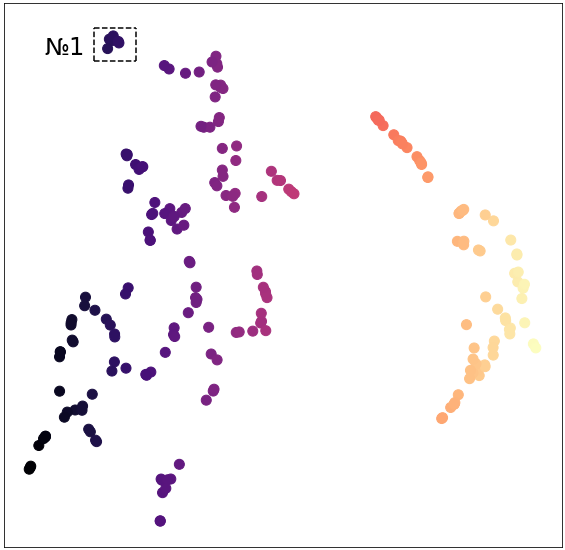
\includegraphics[width=0.85\linewidth]{show.png}\columnbreak
	
	Рассмотрим подробнее результат при \verb|n_neighbors=3| и \verb|min_dist=0.01|. Здесь UMAP рассматривает связь с тремя ближайшими соседями, что позволяет проследить более глубокие взаимосвязи, чем при \verb|n_neighbors=2|. При этом все еще можно различать кластера, то есть можно определить связаны между собой конкретные криптовалюты или нет.
	
	Рассмотрим кластер №1. Исходя из значений двух новых признаков, в данный кластер входят временные ряды: AnarchistsPrime, Einsteinium, GoldBlocks, MonaCoin, TransferCoin, Vertcoin.
\end{multicols}

То есть цены на момент открытия торгов данных криптовалют ведут себя наиболее похоже во времени. Посмотрим на графики цен криптовалют:

\begin{figure}[H]
	\noindent \centering {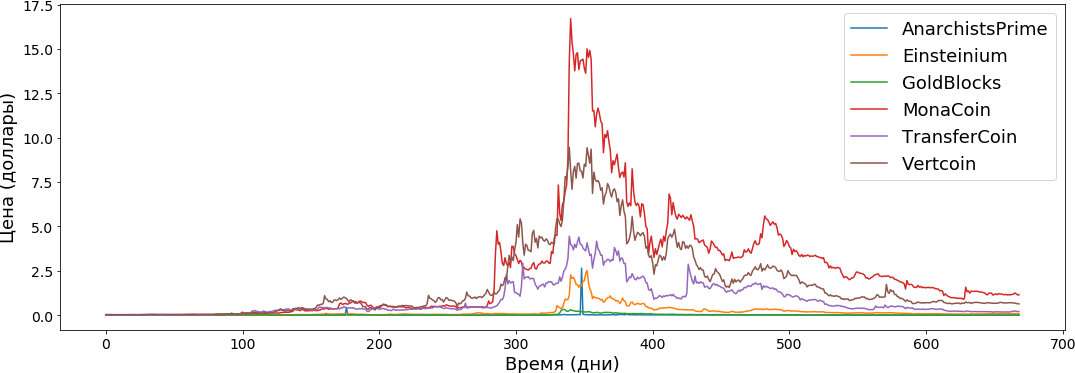
\includegraphics[width = \textwidth]{vecs.png}}
\end{figure}

В самом деле, данные временные ряды имеют похожую динамику. Учитывая стандартизацию данных, они выглядят вот так:

\begin{figure}[H]
	\noindent \centering {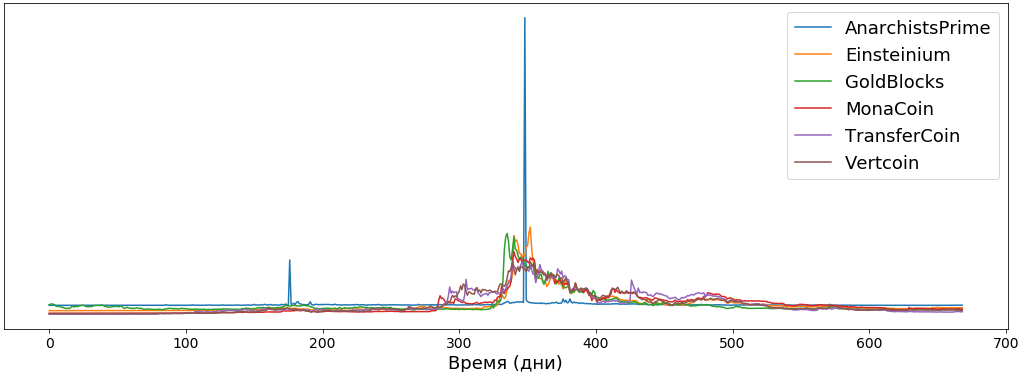
\includegraphics[width = \textwidth]{vecs_s.png}}
\end{figure}

Графики цен криптовалют почти совпадают --- UMAP нашел наиболее похожие ряды, они оказались в одном кластере. Видны небольшие расхождения, например, два внезапных взлета цены AnarchistsPrime. Но если посчитать коэффициенты корреляции, то в целом, ряды сильно коррелируют между собой:

\begin{figure}[H]
	\noindent \centering {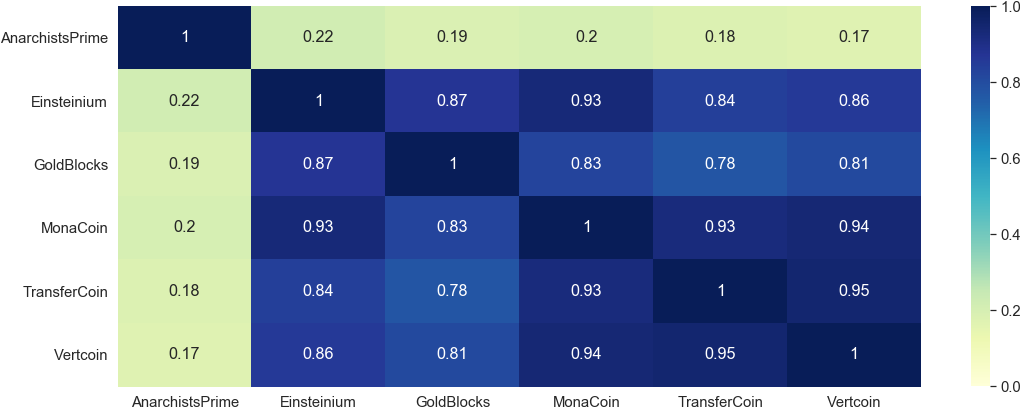
\includegraphics[width = \textwidth]{corr.png}}
\end{figure} 

AnarchistsPrime выбивается из группы криптовалют, имея самые низкие коэффициенты корреляции по сравнению с другими. Как же так получилось, что он оказался в одном кластере с данными рядами?

Ранее мы говорили о том, что расстояния в UMAP и коэффициент корреляции по-разному оценивают схожесть рядов. В этом случае так и вышло. Посчитаем корреляцию между AnarchistsPrime и остальными криптовалютами и найдем наибольший коэффициент:

\begin{figure}[H]
	\noindent \centering {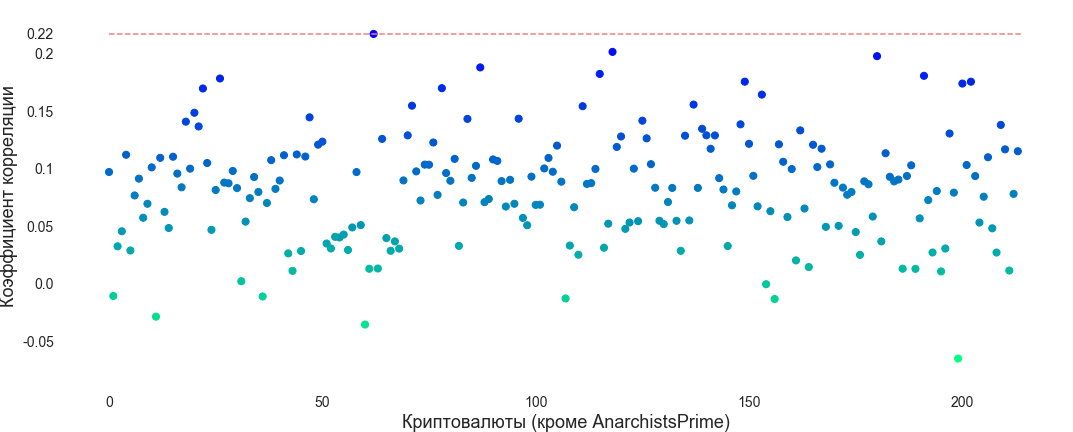
\includegraphics[width = \textwidth]{anarchy.png}}
\end{figure} 

Наибольший коэффициент корреляции временного ряда AnarchistsPrime с другими принимает значение $0.22$ --- корреляция с временным рядом Einsteinium. То есть изменения цены Einsteinium оказались наиболее похожи на поведение AnarchistsPrime, поэтому они оказались в одном кластере. Следующие по схожести ряды также находятся с ним в кластере и имеют чуть меньшие коэффициенты корреляции.
\newpage
\begin{multicols}{2}
	\fbox{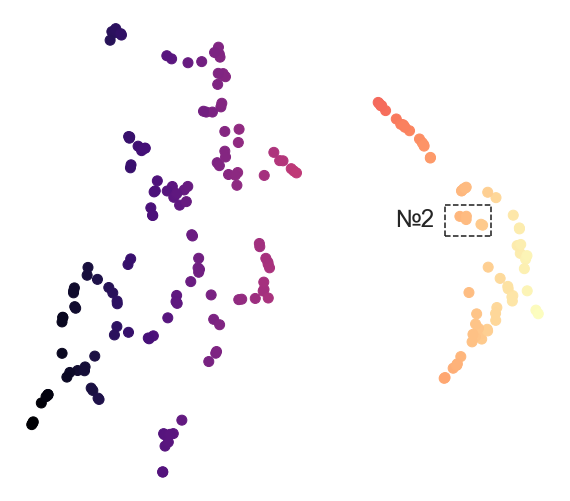
\includegraphics[width=0.85\linewidth]{showy.png}\columnbreak}
	
	Можно также рассмотреть еще один кластер --- желтый (№2). В него входят пять рядов: Augur, Bullion, Decred, Ethereum, Unobtanium.
\end{multicols}

Посмотрим на их графики:

\begin{figure}[H]
	\noindent \centering {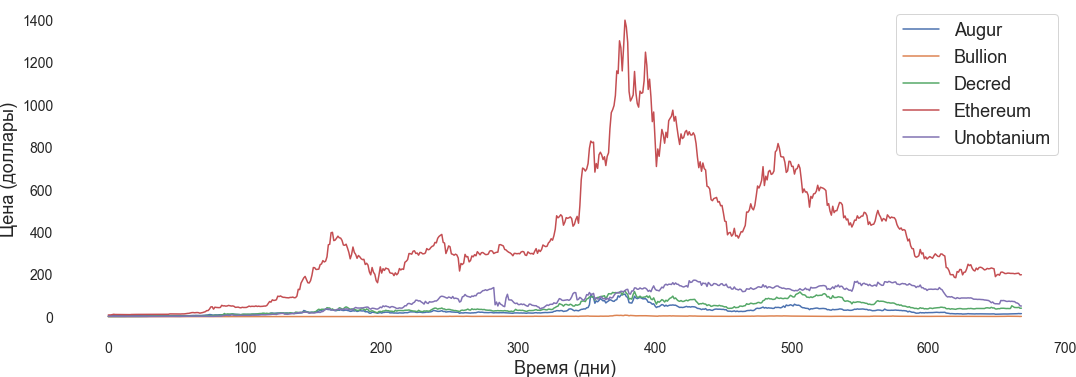
\includegraphics[width = \textwidth]{nvecs.png}}
\end{figure}

Из-за сильной разницы в ценах, особенно с Ethereum, сложно увидеть похожее поведение временных рядов. Построим график со стандартизированными ценами:

\begin{figure}[H]
	\noindent \centering {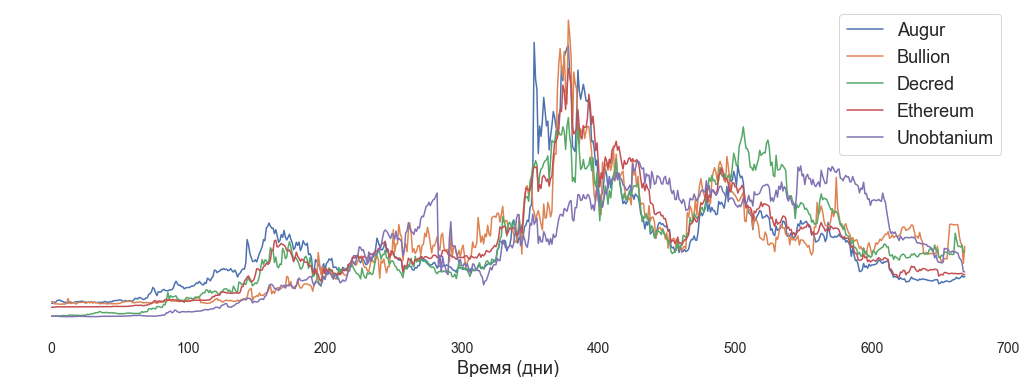
\includegraphics[width = \textwidth]{nvecs_s.png}}
\end{figure}
\newpage
Несмотря на небольшие расхождения, видно, что во многом колебания цен совпадают --- графики накладываются друг на друга. И коэффициенты корреляции принимают большие значения:

\begin{figure}[H]
	\noindent \centering {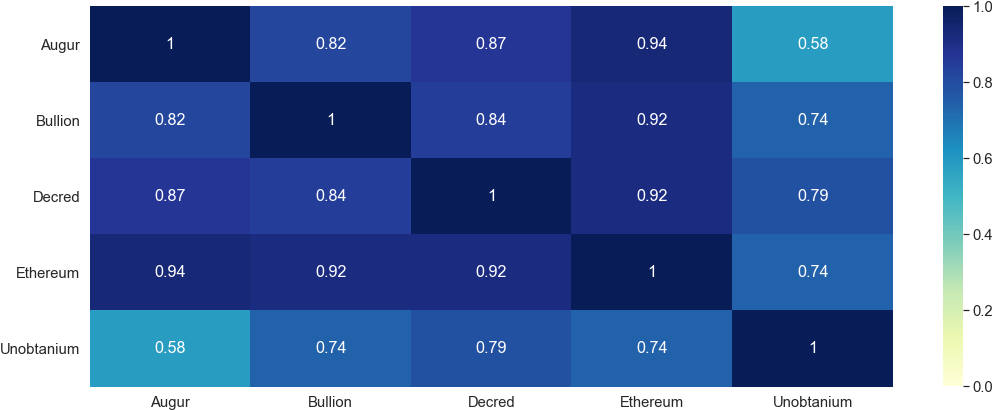
\includegraphics[width = \textwidth]{ncorr.png}}
\end{figure} 

В кластере №2 по сравнению с кластером №1 коэффициенты корреляции не так сильно расходятся во мнении относительно схожести рядов с расстояниями в UMAP.

Мы рассматривали объекты в одном кластере, коэффициенты корреляции между ними принимали большие значения. Но что происходит с объектами, коэффициент корреляции между которыми отрицательный?

Найдем наименьшее значение коэффициента корреляции между рядами. Ему соответствуют ряды AurumCoin и NuBits. Коэффициент корреляции между ними примерно равен $-0.71$. Найдем их на нашей картинке:

\begin{multicols}{2}
	\fbox{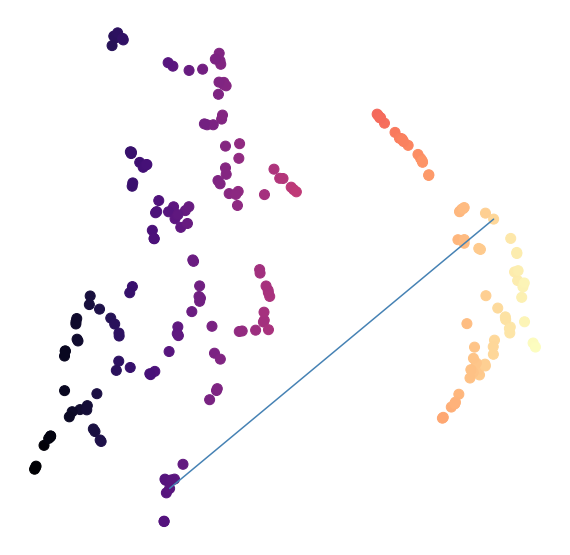
\includegraphics[width=0.85\linewidth]{noncor.png}\columnbreak}
	
	Объекты находятся далеко друг от друга, но некоторые точки лежат на еще большем расстоянии друг от друга. Поскольку изображение, которое мы рассматриваем, было построено для трех ближайших соседей, то UMAP вовсе не учитывал, где будут лежать объекты, являющиеся самыми дальними соседями от исследуемого объекта (для UMAP они даже не являются соседями) --- они отдалились за счет того, что не имеют общих соседей.
\end{multicols}
\newpage
В примере с небольшим количеством рядов мы показали, что коэффициент корреляции отличается от расстояний в UMAP. Посмотрим, что происходит при большом количестве объектов:

\begin{figure}[H]
	\noindent \centering {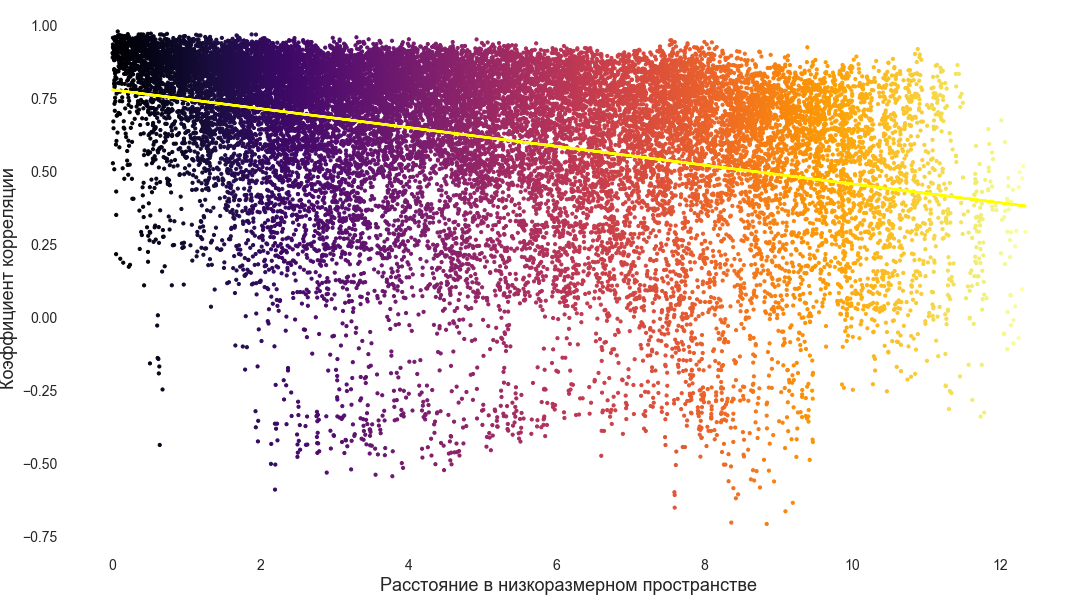
\includegraphics[width = \textwidth]{chart.png}}
\end{figure}

Вновь не видно явной зависимости между коэффициентом корреляции и расстояниями в UMAP --- можно заметить лишь, что при большом коэффициенте корреляции и маленьком расстоянии плотность точек больше, чем в обратной ситуации.

При этом линия тренда имеет отрицательный наклон, как и раньше. И это можно объяснить: UMAP учитывает схожесть тех рядов, которые имеются в выборке, и если совпадает так, что ряды действительно сильно коррелируют, то считает их похожими. Корреляция же измеряет схожесть независимо от других рядов. Поэтому чем больше корреляция, тем меньше расстояние между объектами (потому что они похожи). Но это не работает в обратную сторону: маленькое расстояние между объектами не говорит о сильной корреляции между ними.

Итак, снижение размерности с помощью UMAP и визуализация результатов позволяет взглянуть на внутренние закономерности, существующие в данных.